%%%%%%%%%%%%%%%%%%%%%%%%%%%%%%%%%%%%%%%%%
% "ModernCV" CV and Cover Letter
% LaTeX Template
% Version 1.3 (29/10/16)
%
% This template has been downloaded from:
% http://www.LaTeXTemplates.com
%
% Original author:
% Xavier Danaux (xdanaux@gmail.com) with modifications by:
% Vel (vel@latextemplates.com)
%
% License:
% CC BY-NC-SA 3.0 (http://creativecommons.org/licenses/by-nc-sa/3.0/)
%
% Important note:
% This template requires the moderncv.cls and .sty files to be in the same 
% directory as this .tex file. These files provide the resume style and themes 
% used for structuring the document.
%
%%%%%%%%%%%%%%%%%%%%%%%%%%%%%%%%%%%%%%%%%

%----------------------------------------------------------------------------------------
%	PACKAGES AND OTHER DOCUMENT CONFIGURATIONS
%----------------------------------------------------------------------------------------

\documentclass[10pt,a4paper,sans,unicode,colorlinks,urlcolor=blue]{moderncv} % Font sizes: 10, 11, or 12; paper sizes: a4paper, letterpaper, a5paper, legalpaper, executivepaper or landscape; font families: sans or roman

\moderncvstyle{classic} % CV theme - options include: 'casual' (default), 'classic', 'oldstyle' and 'banking'
\moderncvcolor{blue} % CV color - options include: 'blue' (default), 'orange', 'green', 'red', 'purple', 'grey' and 'black'

\usepackage{lipsum} % Used for inserting dummy 'Lorem ipsum' text into the template

\usepackage{graphicx}

\nopagenumbers{} % uncomment to suppress automatic page numbering for CVs longer than one page

\usepackage[top=0.5in,bottom=0.5in,scale=0.9]{geometry} % Reduce document margins

\usepackage{fontspec} % moderncv themes

\usepackage{xcolor} % Example: \textcolor{red}{text}

\setlength{\hintscolumnwidth}{3cm} % Uncomment to change the width of the dates column

\setlength{\makecvtitlenamewidth}{11cm} % For the 'classic' style, uncomment to adjust the width of the space allocated to your name

\usepackage{pdfpages}
\usepackage{graphicx}
\usepackage{attachfile}

\usepackage{xeCJK}
\ifdefined\setCJKmainfont
  \setCJKmainfont{Noto Serif CJK JP}
\fi
\ifdefined\setCJKsansfont
  \setCJKsansfont{Noto Sans CJK JP}
\fi
\ifdefined\setCJKmonofont
  \setCJKmonofont{Noto Sans Mono CJK JP}
\fi

%----------------------------------------------------------------------------------------
%	NAME AND CONTACT INFORMATION SECTION
%----------------------------------------------------------------------------------------

\firstname{Britt} % Your first name
\familyname{Christy} % Your last name

% All information in this block is optional, comment out any lines you don't need
\title{Spacecraft Flight Software Engineer}
\address{333 Richmond St Apt 2}{El Segundo, CA 90245}
\mobile{(805)-453-9049}
\email{britt.k.christy@gmail.com}
\homepage{www.linkedin.com/in/brittchristy/}{linkedin.com/in/brittchristy/} % The first argument is the url for the clickable link, the second argument is the url displayed in the template - this allows special characters to be displayed such as the tilde in this example
%\extrainfo{\textit{\textcolor{red}{Active TS Clearance - October 2028}}}
\photo[70pt][0.4pt]{pictures/millennium/pathfinder_deployed} % The first bracket is the picture height, the second is the thickness of the frame around the picture (0pt for no frame)
% \quote{"Successful development and mission operations for any spacecraft depend heavily on flight software/firmware/gateware to interface avionics and humans. I’m grateful (and extremely lucky) for the opportunities I’ve been given to develop and own multiple flight software systems from cradle-to-grave ... \textbf{8 successful spacecraft and still counting!}" - Britt Christy}

% \quote{"Successful development and mission operations for any spacecraft depend on flight software."}

%----------------------------------------------------------------------------------------

\begin{document}

%----------------------------------------------------------------------------------------
%	COVER LETTER
%----------------------------------------------------------------------------------------

% To remove the cover letter, comment out this entire block

% \clearpage

% \recipient{HR Department}{Corporation\\123 Pleasant Lane\\12345 City, State} % Letter recipient
% \date{\today} % Letter date
% \opening{Dear Sir or Madam,} % Opening greeting
% \closing{Sincerely yours,} % Closing phrase
% \enclosure[Attached]{curriculum vit\ae{}} % List of enclosed documents

% \makelettertitle % Print letter title

% \lipsum[1-2] % Dummy text
% \lipsum[4] % Dummy text

% \makeletterclosing % Print letter signature

% \newpage

%----------------------------------------------------------------------------------------
%	CURRICULUM VITAE
%----------------------------------------------------------------------------------------

\makecvtitle % Print the CV title
\small

%----------------------------------------------------------------------------------------
%	TECHNOLOGIES SECTION
%----------------------------------------------------------------------------------------

\section{Technologies}
\cvitem{Languages}{Embedded C/C++ \textit{(RT Linux, FreeRTOS)}, Python, Verilog, LabVIEW Real-Time/FPGA, basic bash scripting, x86 Assembly, \LaTeX, MatLab, \textit{Willing to learn Rust}}
\cvitem{Hardware}{Xilinx Ultrascale+ SoC (ZCU102), STM32H753 Arm Cortex-M4/M7 microcontroller, Microsemi FPGA, NI-SBRIO9651 (Zynq-7000)}
\cvitem{Debug Tools}{gdb, Saleae (logic analyzer), Segger JLink debugger, good old fashioned print statements}
\cvitem{Development Tools}{RT Linux, Gitlab/Gitlab CI, VSCode, enough VIM to not be crippled on a headless machine, Saleae, Segger JLink, STM32, Vivado/Petalinux, Libero/ModelSim, LabVIEW Real-Time/FPGA, Pycharm, Eclipse (if really necessary)}
\cvitem{Serial Protocols}{UART (RS485/RS422), SPI, I2C, CAN, a bit of SpaceWire}
\cvitem{Avionics Driver software/FPGA}{Reaction Wheels (multiple serial protocols and bus configurations), ADC, GPS, IMU, TAM, ETC (torque coils), Prop, Spacecraft Clock (FPGA)}
\cvitem{Flightware Miscellaneous}{Packet processing (90\% of job), GNC model interfaces, ATS/RTS command sequences, historical/RT telemetry, error logging, command handling, telemetry marshalling, fault management, python scripted command/telemetry code generation for serialization/deserialization and fault management, HITL Testing, mission operations support}
\cvitem{Electronics Skills}{Soldering, crimping, wiring, breadboarding, hardware debugging with logic analyzer, grokking schematics and hardware ICDs}

%----------------------------------------------------------------------------------------
%	WORK EXPERIENCE SECTION
%----------------------------------------------------------------------------------------

\section{Work and Research Experience}

% \subsection{Vocational}

% \cventry{2010--2011}{}{}{}{}{Spent some time finding myself. This was a courageous endeavour that didn't have a job title. It was quite important to my overall development though so I'm adding it to my CV. Also it explains the gap in my otherwise stellar CV.}

% True Anomaly
\cventry{July 2025--Oct 2025\newline{\textit{(~3 months)}}\newline\newline
\includegraphics[height=22pt]{pictures/true_anomaly_logo.jpg}}{Senior Flight Software Engineer}{\textsc{True Anomaly Space}}{Long Beach}{California}{
\begin{itemize}
\item ZCU102 Test Setup for radio talking TCP/IP over a TUN interface via HDLC over LVDS:
% \item Goal was to get teammate's high-level radio driver working with firmware for portable radiation test setup
% \item Set up ESD-safe workspace for personal ZCU102 devkit
\item Set up ESD-safe workspace for ZCU102 devkit
\item Organized and version-controlled most useful schematics and ICDs
\item Installed Vivado, Vitis, and System Controller on Windows, WSL2, and Linux VMs
\item Made twisted-pair LVDS clock and data cables for loopback 
\item Configured LVDS clocks and voltages via System Controller for HDLC signaling
\item Set up Saleae logic analyzer to probe LVDS loopback via XM105 FPGA debug breakout board
\item Got ZCU102 booting over debug UART
\item Patched legacy U-Boot dtc lexer/parser to newer version and rebuilt firmware stack (U-Boot, kernel, DTB, rootfs) to fix build errors 
\item Modified rootfs overlay to enable static IP for SSH access
% \item My employment ended prematurely despite steady technical progress and a clear roadmap to completion.
\item The work planned for the remainder of October was well-defined to deliver a working radio test setup:
\begin{itemize}
% \item Update FPGA build from 2019.2 → 2022.1 and resolve synthesis issues
\item Update FPGA build to newer version to resolve synthesis issues
% \item Validate LVDS mapping and HDLC waveform integrity via loopback
\item Validate bytes in software and with logic analyzer (Application layer -> DMA FIFO -> HDLC -> FPGA breakout board)
\item Make filesystem stick after reboot
\item Get flight software application running
\item Integrate and test radio driver with real radio
\end{itemize}
\end{itemize}}

% Millennium round 2
\cventry{Sep 2023--Mar 2025\newline{\textit{(1 year, 7 months)}}\newline\newline
\includegraphics[height=22pt]{pictures/millennium/millennium_space_systems_logo.jpg}}{Senior Spacecraft Software Engineer IV}{\textsc{Millennium Space Systems}}{El Segundo}{California}{
\begin{itemize}
\item Developed reaction wheel driver for two RS485 busses of 3 reaction wheels each (including hardware purchasing, contract negotiation, avionics interfaces, relationship building with the vendor, etc before design)
\item Demonstrated driver design, command/telemetry interface definition, full unit test coverage, driver connected to emulator on SIL with real flightlike ground software and GNC/plant models
% \item Documented next steps for updates to test with real hardware on ZCU102, flatsat, flight and iterating/retesting driver/emulator on HITL/SIL until ops agrees that the system is behaving in a flightlike manner (or close enough)
\item Wrote helper tool/script for unit test coverage to make it easy to run locally
\item Got legacy version of Vivado working in WSL2 to avoid horrible delay when X11 forwarding GUI running on shared Linux VM
\begin{itemize}
    \item Most stuff can be TCL scripted, but sometimes the GUI is better.
\end{itemize}
% \item Advised flight software microcontroller team to make the switch from Keil IDE to Cmake + VsCode + JLink debugger + Catch2 unit testing
% \item Convinced new programs that success requires investing in multiple HITLs (hardware in the loops) as well as SIL (software in the loops) (need both, not one or the other) \item Educated new program managers on the value of providing flight software with devkits and extra hardware when possible to speed up HITL development prior to flatsat/flight integration
% \item Influenced the decision to grant flight software additional lab space for new FSW HITLs
% \item Encouraged learning how to bring code up on hardware devkits while HITLs were getting built up rather than only relying on the SIL
% \item Negotiated agreement with team to start adding human-readable flight software documentation to codebase (not just doxygen) to help ops and new FSW folks for onboarding and remind OG folks how legacy flight software works during ops.
% \item Taught new folks that documentation isn't just for operators - its a selfish thing to make life easier for your future self when you have to patch bugs during operations or start forgetting how things work
% \item Supported recruiting, teambuilding and onboarding of new systems and firmware/software engineers for several new programs with overlapping firmware and hardware requirements.
% \item Helped transition and onboard a newgrad to a payload development team
% \item Helped get a contractor to join the team officially and start doing excellent work on a radio interface
\end{itemize}}

%------------------------------------------------

% Turion
\cventry{Jun 2023--Jul 2023\newline{}\textit{(2 months)}\newline{}\newline{}
\includegraphics[height=20pt]{pictures/turion_space_logo.jpg}}{Senior Spacecraft Flight Software Engineer (Contractor)}{\textsc{Turion Space}}{Irvine}{California}{
\begin{itemize}
\item Helped commission Turion's first spacecraft during initial operations.
\item Coded and breadboarded GPS hardware emulator to troubleshoot and identify root cause of time sync anomaly
\item Helped identify and mitigate anomalies with GPS and RWA
% \item Drove vendor negotiations for on-orbit software updates and fixes
\item Created and executed pass plans with mission operatrs
\item Wrote, tested, uploaded, executed, and downlinked logs for stored command sequences to validate hardware and command interfaces in flight
\item Demonstrated the importance of onboard command sequences to “fly like you test”, increase determinism, minimize human error, and maximize the amount of information gathered during quick LEO passes
% \item Taught best practices for HITL and flatsat testbed architecture to support pipelined avionics/flight/ground software development, simplify configuration management, and minimize resource contention throughout integration, test, and mission operations
% \item Participated in flight software requirements discussions for Droid 2
\end{itemize}}

% Inversion
\cventry{Mar 2022--Jun 2023\newline{}\textit{(1 year, 4 months)}\newline{}
\includegraphics[height=35pt]{pictures/inversion_space_logo.jpg}}{Senior Spacecraft Flight Software Engineer}{\textsc{Inversion Space}}{Torrance}{California}{ 
\begin{itemize}
\item Built reusable reentry vehicle tech demo named Ray (flew in 2025): 
\emph{\href{https://www.inversionspace.com/ray}{reentry vehicle mission}}
\item Wrote flight software infrastructure in C++ with FreeRTOS on STM32 microprocessor 
\item Configured and purchased avionics flight computer stack and flatsat testbed hardware
\item Negotiated flight software and mission operations training purchases with vendor
\item Set up initial ground software with flatsat
\item Set up ISO7/10,000 glovebox and wiring for initial flight hardware testing of reaction wheels and startracker
\item Configured, negotiated, purchased, and completed initial hardware setup and self testing for closed loop HITL hardware
\item Recruited and interviewed extensively for flight software, avionics, and HITL developers
% \item Planned and led initial development of GNC-FSW interface architecture and HITL
\item Built out initial avionics lab and avionics testing interfaces and purchased tools and supplies
\item Set up GitLab repos and CI for flight software builds with static IPs
\item Onboarded avionics engineer and worked with them to design embedded flight software architecture and board interfaces 
% \item Broke down flight software and ground software development into tasks and timeline 
% \item Taught spacecraft flight software and Mission Control software architecture 
\item Negotiated software updates and bug fixes with vendor
\item Got serial interfaces working for all drivers
\item Onboarded flight software interns to write reaction wheel and radio drivers
\end{itemize}}

%------------------------------------------------

% Millennium 1 (don't forget NI awards)

\cventry{Mar 2019--Mar 2022\newline{\textit{(3 years, 1 month)}\newline\newline
\includegraphics[height=22pt]{pictures/millennium/millennium_space_systems_logo.jpg}}}{Senior Spacecraft Flight Software Engineer}{\textsc{Millennium Space Systems}}{Los Angeles}{}{
\begin{itemize}
% \item Extensively documented and applied and taught lessons learned from Altair Pathfinder mission operations to avoid making the same mistakes again 
% \item Iterated on Altair-Pathfinder based flight software (this time with a larger team) from concept to deployment for multiple iterations of vehicles and constellations spanning several programs, including DARPA's Redeye constellation: \emph{\href{https://spacenews.com/millennium-space-reveals-results-of-darpas-red-eye-smallsat-experiment/}{https://spacenews.com/millennium-space-reveals-results-of-darpas-red-eye-smallsat-experiment/}}
\item Iterated with team on my original flight computer software for a Customer: \emph{\href{https://spacenews.com/millennium-space-reveals-results-of-darpas-red-eye-smallsat-experiment/}{experimental mission}}
\item Supported mission operations, anomaly troubleshooting, and on-orbit software patches for multiple vehicles and missions as both flight software REA and individual contributor while continuing to maintain large percentage of code ownership.
\item Developed core Gitlab CI and LabVIEW/C++ code generation from "one source of truth" for shared command, telemetry, and other interfaces common to all missions
\item Developed regression testing infrastructure, CHANGELOG, and various other configuration management bits and bobs to validate, document, and version new flight software builds
% \item Refactored common infrastructure/code into shared flight software codebases with lots of autogeneration to support multiple iterations of overlapping missions, vehicles, and constellations with minimal effort
% \item Wrote propulsion system driver, GNC interfaces, and test procedures
% \item Led vendor negotiations to fix bugs with propulsion system and hardware emulator
% \item Developed mission ops training for prop system and contributed to CONOPs
\item Co-wrote propulsion system driver and supported testing, debugging and fixing issues with it all the way through successful integration with the flight vehicle
% and initial mission operations
% \item Contributed to a new pure-C/C++ core flight software code base for various smallsat programs, including the GPS driver for NASA’s TRACERS heliophysics mission: \emph{\href{https://spacenews.com/millennium-space-delivers-two-spacecraft-for-upcoming-nasa-mission/}{https://spacenews.com/millennium-space-delivers-two-spacecraft-for-upcoming-nasa-mission/}}
\item Wrote GPS driver for NASA heliophysics science mission (flew in 2025): \emph{\href{https://spacenews.com/millennium-space-delivers-two-spacecraft-for-upcoming-nasa-mission/}{heliophysics mission}}
\item Contributed to first iteration of guidelines for embedded real-time C/C++ flight software to increase determinism and reliability in space, make bugs easy to identify and patch, conserve limited resources, and improve interfaces and documentation for our mission operators.
% \item Interviewed, onboarded, and tasked new engineers to grow our team.
% \item Code reviewed and coordinated tasks to fix anomalies found during flight, and applied updates to both vehicles on orbit and new vehicles under development on the ground.
% \item Wrote a spacecraft-to-host-vehicle interface firmware for microsemi FPGA to translate spacecraft command/telemetry packet byte stream to host vehicle LDPE packets (similar to existing ESPA ring protocols.)
\item Wrote a spacecraft-to-host-vehicle interface firmware for microsemi FPGA to translate spacecraft command/telemetry packet byte stream to proprietary host vehicle packets
\end{itemize}}

%------------------------------------------------

% Millennium 0
\cventry{Jun 2015--Mar 2019\newline{\textit{(3 years, 10 months)}\newline\newline
\includegraphics[height=22pt]{pictures/millennium/millennium_space_systems_logo.jpg}}}{Spacecraft Avionics Software Engineer}{\textsc{Millennium Space Systems}}{Los Angeles}{}{
\begin{itemize}
 \item Wrote 90\% of the real-time flight software and FPGA gateware for one of the flight computers on the Altair Pathfinder tech demo:
 \item \emph{\href{https://www.prnewswire.com/news-releases/millennium-space-systems-altair-pathfinder-satellite-surpasses-10-000-hours-in-orbit-300685534.html}{pathfinder-satellite-surpasses-10-000-hours-in-orbit}}
 \item \emph{\href{https://spacenews.com/millennium-space-systems-completes-successful-altair-pathfinder-mission/}{successful-altair-pathfinder-mission}}
\item Wrote and integrated low-level FPGA and high-level RT Linux drivers using LabVIEW FPGA, LabVIEW Real Time (Linux RT under the surface), and C++ for various avionics (GPS, startrackers, reaction wheels, three-axis-magnetometer, ETC (Electromagnetic Torque Coils), FPGA spacecraft clock).
\item Coded flight software infrastructure (command sequences, command/telemetry management, etc)
\item Wrote FPGA hardware emulators to test the drivers
\item Wrote code to serialize and deserialize commands and telemetry
\item Collaborated with avionics integration and test engineers and GNC/OPS for rigorous testing on HIL, flatsat, and flight vehicle (no SIL at the time)
% \item Developed Altair Ground Interface in LabVIEW to test the flight software before we had a real ground software devleoper to take over
\item Supported Altair Pathfinder team throughout initial mission operations
\item Gained experience debugging and patching flight software on orbit
\item Contributed to paper written by Altair Pathfinder team to share lessons learned from on-orbit troubleshooting
\item Created initial Gitlab CI build system to tie together tools and versioning and configuration management
\item Built tool to autogenerate GNC command, telemetry, and interface code as well as various other flight software interfaces and documentation from Simulink models
\end{itemize}}

%------------------------------------------------

% \subsection{Internships \& Undergrad Research}

% % undergrad research
% \cventry{Spring 2015}{Undergrad Research}{}{University of California, Santa Barbara}{}{
% \begin{itemize}
%     \item Contributed a bit to a standard library for a python tool called PyRTL to design and simulate digital circuits and compile to verilog.
%     \item gitlab repo: \emph{\href{https://github.com/UCSBarchlab/PyRTL}{https://github.com/UCSBarchlab/PyRTL}}
% \end{itemize}
% }

%------------------------------------------------

% capstone
\cventry{Winter--Spring 2015}{Senior Engineering Capstone Project}{}{University of California, Santa Barbara}{}{
\begin{itemize}
 \item Developed the back end for a video conferencing web application using Ruby on Rails, with a voice-activated smart assistant named Benedict to provide helpful services during a meeting.
\item Benedict used a natural language processing model trained to scrape the Internet for information from popular websites.
% \item \textit{Sound familiar?} ChatGPT was also created in 2015...
\item Won first prize (see link for document downloads): \emph{\href{https://capstone.cs.ucsb.edu/past15ws.html}{https://capstone.cs.ucsb.edu/past15ws.html}}
% \item Webapp link: \emph{\href{benedictation.io}{benedictation.io}}
\item Github link: \emph{\href{https://github.com/Team-Struct-by-Lightning/Benedictation}{https://github.com/Team-Struct-by-Lightning/Benedictation}}
\end{itemize}}

% Internships

%------------------------------------------------

% Liaison Technologies
\cventry{Fall 2014 \textit{(1 year)}}{Intern}{Liaison Technologies (Quality Assurance)}{Santa Barbara}{California}{
\begin{itemize}
    \item Performed quality assurance for data integration products designed by Liaison.
\end{itemize}
}

%------------------------------------------------

% Caltech LIGO

\cventry{Summer 2014 \newline{\textit{(3 months)}}}{Intern}{Caltech LIGO (Laser Interferometer Gravitational Wave Observatory)}{Pasadena}{California}{
\begin{itemize}
\item Wrote Matlab code which used Baysian inference to analyze simulated observational data from correlated gravitational wave detectors in order to estimate parameters such as neutron star formation rate density throughout the universe.
\item Research Paper: \emph{\href{https://dcc.ligo.org/public/0115/P1400199/001/BrittChristyFinalPaper.pdf}{https://dcc.ligo.org/public/0115/P1400199/001/BrittChristyFinalPaper.pdf}}
\item Research Presentation Charts: \emph{\href{https://dcc.ligo.org/public/0115/G1400897/001/brittChristyFinalPresentation.pdf}{https://dcc.ligo.org/public/0115/G1400897/001/brittChristyFinalPresentation.pdf}}
\item The first detection was announced 2 years later on February 11 2016 confirming the merger of two black holes.
\end{itemize}}

%------------------------------------------------

% % Experimental Astrophysics Lab
% \cventry{Fall 2013\newline{\textit{(3 months)}}}{Student Researcher}{University of California, Santa Barbara Experimental Astrophysics Lab}{}{}{
% \begin{itemize}
%     \item Debugged Java control code for a morphable mirror telescope which used a laser tracker and actuators to actively correct for deviations from the desired mirror surface.
% \end{itemize}}

%------------------------------------------------

% Tyndall Ireland
\cventry{Summer 2012\newline{\textit{(3 months)}}}{Intern}{Tyndall National Institute (Quantum Transport Simulation)}{Cork, Ireland}{}{
\begin{itemize}
\item Developed a multi-platform desktop application graphical user interface for a quantum transport simulation program using Java SWT.
\item Project abstract: \emph{\href{https://mrlweb.mrl.ucsb.edu/education/undergrad/cisei/2012/brittany-christy}{https://mrlweb.mrl.ucsb.edu/education/undergrad/cisei/2012/brittany-christy}}
\end{itemize}}

%------------------------------------------------

% Private Java Tutor
% \cventry{Spring 2012}{Private Java Tutor}{Self-employed}{Santa Barbara}{}{
% \begin{itemize}
% \item Taught the basics of the Java programming language, as well as object oriented design principles to high school students.
% \end{itemize}
% }

%------------------------------------------------

% CS lab TA
% \cventry{Spring 2012}{Substitute Lab Teaching Assistant}{Santa Barbara City College Computer Science Lab}{Santa Barbara}{}{
% \begin{itemize}
% 	\item Helped students debug and verify programming assignments.
% 	\item Shut down the lab at closing time.
% \end{itemize}
% }

%------------------------------------------------

% Experimental Astrophysics Lab Dewars
\cventry{Summer 2011\newline{\textit{(4 months)}}}{Intern}{University of California, Santa Barbara Experimental Astrophysics Lab}{Santa Barbara}{}{%
   \begin{itemize}
   \item Worked on project for a microwave telescope called "LATTE" (Low Frequency All-sky TemperaTure Experiment) to study frequencies from the plane of our milky way galaxy - both to better understand them, and to subtract them from the CMB to reduce noise.
	\item Contributed to design and test of experimental microwave telescope components such as the cryogenic dewar needed to insulate the signal amplifier from thermal noise.
	\item Simulated radiative heat flux and calculated radiative heat transfer characteristics for various dewar geometries using SolidWorks and Mathematica.
\end{itemize}}

%------------------------------------------------

% % \subsection{Miscellaneous}

% Novel Cafe
% \cventry{2010-2011}{Barista}{Starbucks}{Santa Monica}{}{}

%------------------------------------------------

% Starbucks
%\cventry{2009-2010}{Barista}{Novel Cafe}{Santa Monica}{}{}

%------------------------------------------------

% Toothking Dentistry
% \cventry{Fall 2010}{Receptionist}{ToothKing Dentistry}{Santa Monica}{}{
% \begin{itemize}
% \item Calculated patient co-payments for various dental procedures.
% \item Became familiar with various dental procedures and anatomy.
% \end{itemize}}

%------------------------------------------------

% The Coffee Bean
% \cventry{2008-2009}{Barista}{The Coffee Bean and Tea Leaf}{Santa Monica}{California}{}

% AMC movie theatre
% \cventry{2007-2008}{Concessions}{AMC Movie Theatre}{Santa Monica}{California}{}

%----------------------------------------------------------------------------------------
%	EDUCATION SECTION
%----------------------------------------------------------------------------------------

\section{Education}

% usage: \cventry{years}{degree/job title}{institution/employer}{localization}{optional: grade/...}{optional: comment/job description}

\cventry{2012--2015}{B.S. Computer Engineering}{University of California, Santa Barbara - College of Engineering}{Santa Barbara}{}{Member of W.I.S.H. club (Women in Software and Hardware)}

\cventry{2011--2012}{Computer Science \& Programming}{Santa Barbara City College}{Santa Barbara}{}{Computer Science club Vice President}

\cventry{2008--2011}{Physics \& Astronomy}{Santa Monica College}{Santa Monica}{}{Astronomy club Secretary}

% \cventry{2011--2012}{Computer Science \& Programming}{Santa Barbara City College}{Santa Barbara}{GPA: 4.00}{Computer Science club Vice President}

% \cventry{2008--2011}{Physics \& Astronomy}{Santa Monica College}{Santa Monica}{GPA: 3.5}{Astronomy club Secretary}

% \subsection{Courses Completed}
% \cvitem{Mathematics}{Calculus Series, Differential Equations, Linear Algebra, Probability and Statistics, Discrete Mathematics}
% \cvitem{Programming}{C Programming, Java Programming,  C++ Programming, x86 Assembly, MIPS  Assembly, Data Structures with C++, Data Structures with Java, Android Programming, Object Oriented Design Patterns, Operating Systems, Compilers}
% \cvitem{Circuit Design}{Digital Design Principles, Digital Design Methodologies, Circuits and Devices (A,B,C)}
% \cvitem{Circuit Verification}{Digital Design with VHDL and Synthesis, Computer-Aided Design of VLSI Circuits}
% \cvitem{Other}{Networking I/II/III, Databases}


% \section{Masters Thesis}

% \cvitem{Title}{\emph{Money Is The Root Of All Evil -- Or Is It?}}
% \cvitem{Supervisors}{Professor James Smith \& Associate Professor Jane Smith}
% \cvitem{Description}{This thesis explored the idea that money has been the cause of untold anguish and suffering in the world. I found that it has, in fact, not.}

%----------------------------------------------------------------------------------------
%	AWARDS SECTION
%----------------------------------------------------------------------------------------

\section{Awards}

% computer science capstone first place
% NI award

\cvitem{2017}{National Instruments NI Engineering Impact Award for Altair Pathfinder spacecraft tech demo}
\cvitem{2015}{First place in Senior Computer Science Capstone project competition for Benedictation}
% \cvitem{2012, 2013}{Included in University of California Santa Barbara's Dean's Honor Roll.}
% \cvitem{2011}{Included in Santa Barbara City College President's Honor Roll.}

%----------------------------------------------------------------------------------------
%	LANGUAGES SECTION
%----------------------------------------------------------------------------------------

% \section{Languages}
% \cvitemwithcomment{English}{Mothertongue}{I sure hope I'm fluent in the English language by now}
% \cvitemwithcomment{Japanese}{3 years}{Basic words and phrases, can read and write ひらがな and カタカナ}

%----------------------------------------------------------------------------------------
%	INTERESTS SECTION
%----------------------------------------------------------------------------------------

\section{Hobbies and Interests}

\renewcommand{\listitemsymbol}{-~} % Changes the symbol used for lists

Astronomy $\cdot$ Space exploration $\cdot$ Coding $\cdot$ Cooking $\cdot$ Indoor Rock Climbing $\cdot$ Freediving $\cdot$ Gardening $\cdot$ Flying kites

% \cvlistdoubleitem{Piano}{Chess}
% \cvlistdoubleitem{Cooking}{Dancing}
% \cvlistitem{Running}

%----------------------------------------------------------------------------------------

% \section{What I like to work on}
% {
%     \begin{itemize}
%         \item FPGA development of any kind
%         \item Tasks that allow me to learn new skills and new hardware from the bottom up with high levels of ownership
%         \item Avionics drivers
%         \begin{itemize}
%             \item Good avionics drivers start with a clear understanding and implemlentation of both low level hardware interfaces and high level command/telemetry
%             \item I want to implement the low level FPGA/firmware parts of the code too.
%             \item I don't like \textbf{only} being allowed to do high level application software because someone decides that the low level development is "too hard for me" despite my training in digital design and real life experience :)
%         \end{itemize}
%         \item Small glue code/tools/refactoring to make code and testing and operations easier
%         \item supporting mission operations and cleanroom testing
%         \item working with gnc and avionics and ops
%     \end{itemize}
% }

% \section{Work I would rather not do myself again}
% \begin{itemize}
%     \item custom command and telemetry definitions and autogeneration (so important, happy to advise)
%     \item ground databases
%     \item fault management handler
%     \item command sequence handler
%     \item Exclusively SITL/HITL development
%     \begin{itemize}
%         \item writing emulators occasionally is fun, but I am more experienced with writing flight code, and the extra pressure that comes with it motivates me to to my best.
%     \end{itemize}
% \end{itemize}

% \section{Bucket List (what I want to work on someday)}
% {
% \begin{itemize}
%     \item bootloader and linker script
%     \item flash controller
%     \item Microcontroller development with FreeRTOS (only got to scratch the surface at previous jobs)
%     \item motor controller interface (brushless DC, others)
%     \item NASA CFS port
%     \item board bringup for custom flight computer
%     \item spacecraft bus network interface (spacewire, RS485 round robin, CAN, etc - usually FPGA stuff)
%     \item Ethernet/TSN ethernet
%     \begin{itemize}
%         \item \href{https://ntrs.nasa.gov/api/citations/20020039726/downloads/20020039726.pdf}{ethernet for space flight applications [NASA]}
%         \item \href{https://digitalcommons.usu.edu/cgi/viewcontent.cgi?article=1813&context=smallsat}{Conceptual Design of an IP-based Satellite Bus Using Internet
% Technologies}
%         \item \href{https://tsn-network.com/}{TSN ethernet standards}
%         \item \href{https://arxiv.org/pdf/1804.07643}{time-sensitive networking for robotics}
%         \item \href{https://github.com/the-aerospace-corporation/satcat5}{satcat5 router}
%     \end{itemize}
%     \item computer vision
%     \item edge processing on Versals \href{https://www.amd.com/en/products/adaptive-socs-and-fpgas/versal.html}{Versal adaptive-socs-and-fpgas}
%     \item machine learning in FPGA (would love to implement simple neural network)
%     \item analog computer for fast matrix multiplication (like this one: \href{https://mythic.ai/}{https://mythic.ai/}
%     \item PCB design and bringup (not software, but something I want to learn)
%     % \item payload driver - have only done flight computer work, never payload work
%     % \item full hardware emulator (I've done pieces, never the whole thing)
%     % \item gnc control (have never learned how the control algorithms work and would like to)
% \end{itemize}
% }

% \newpage
% 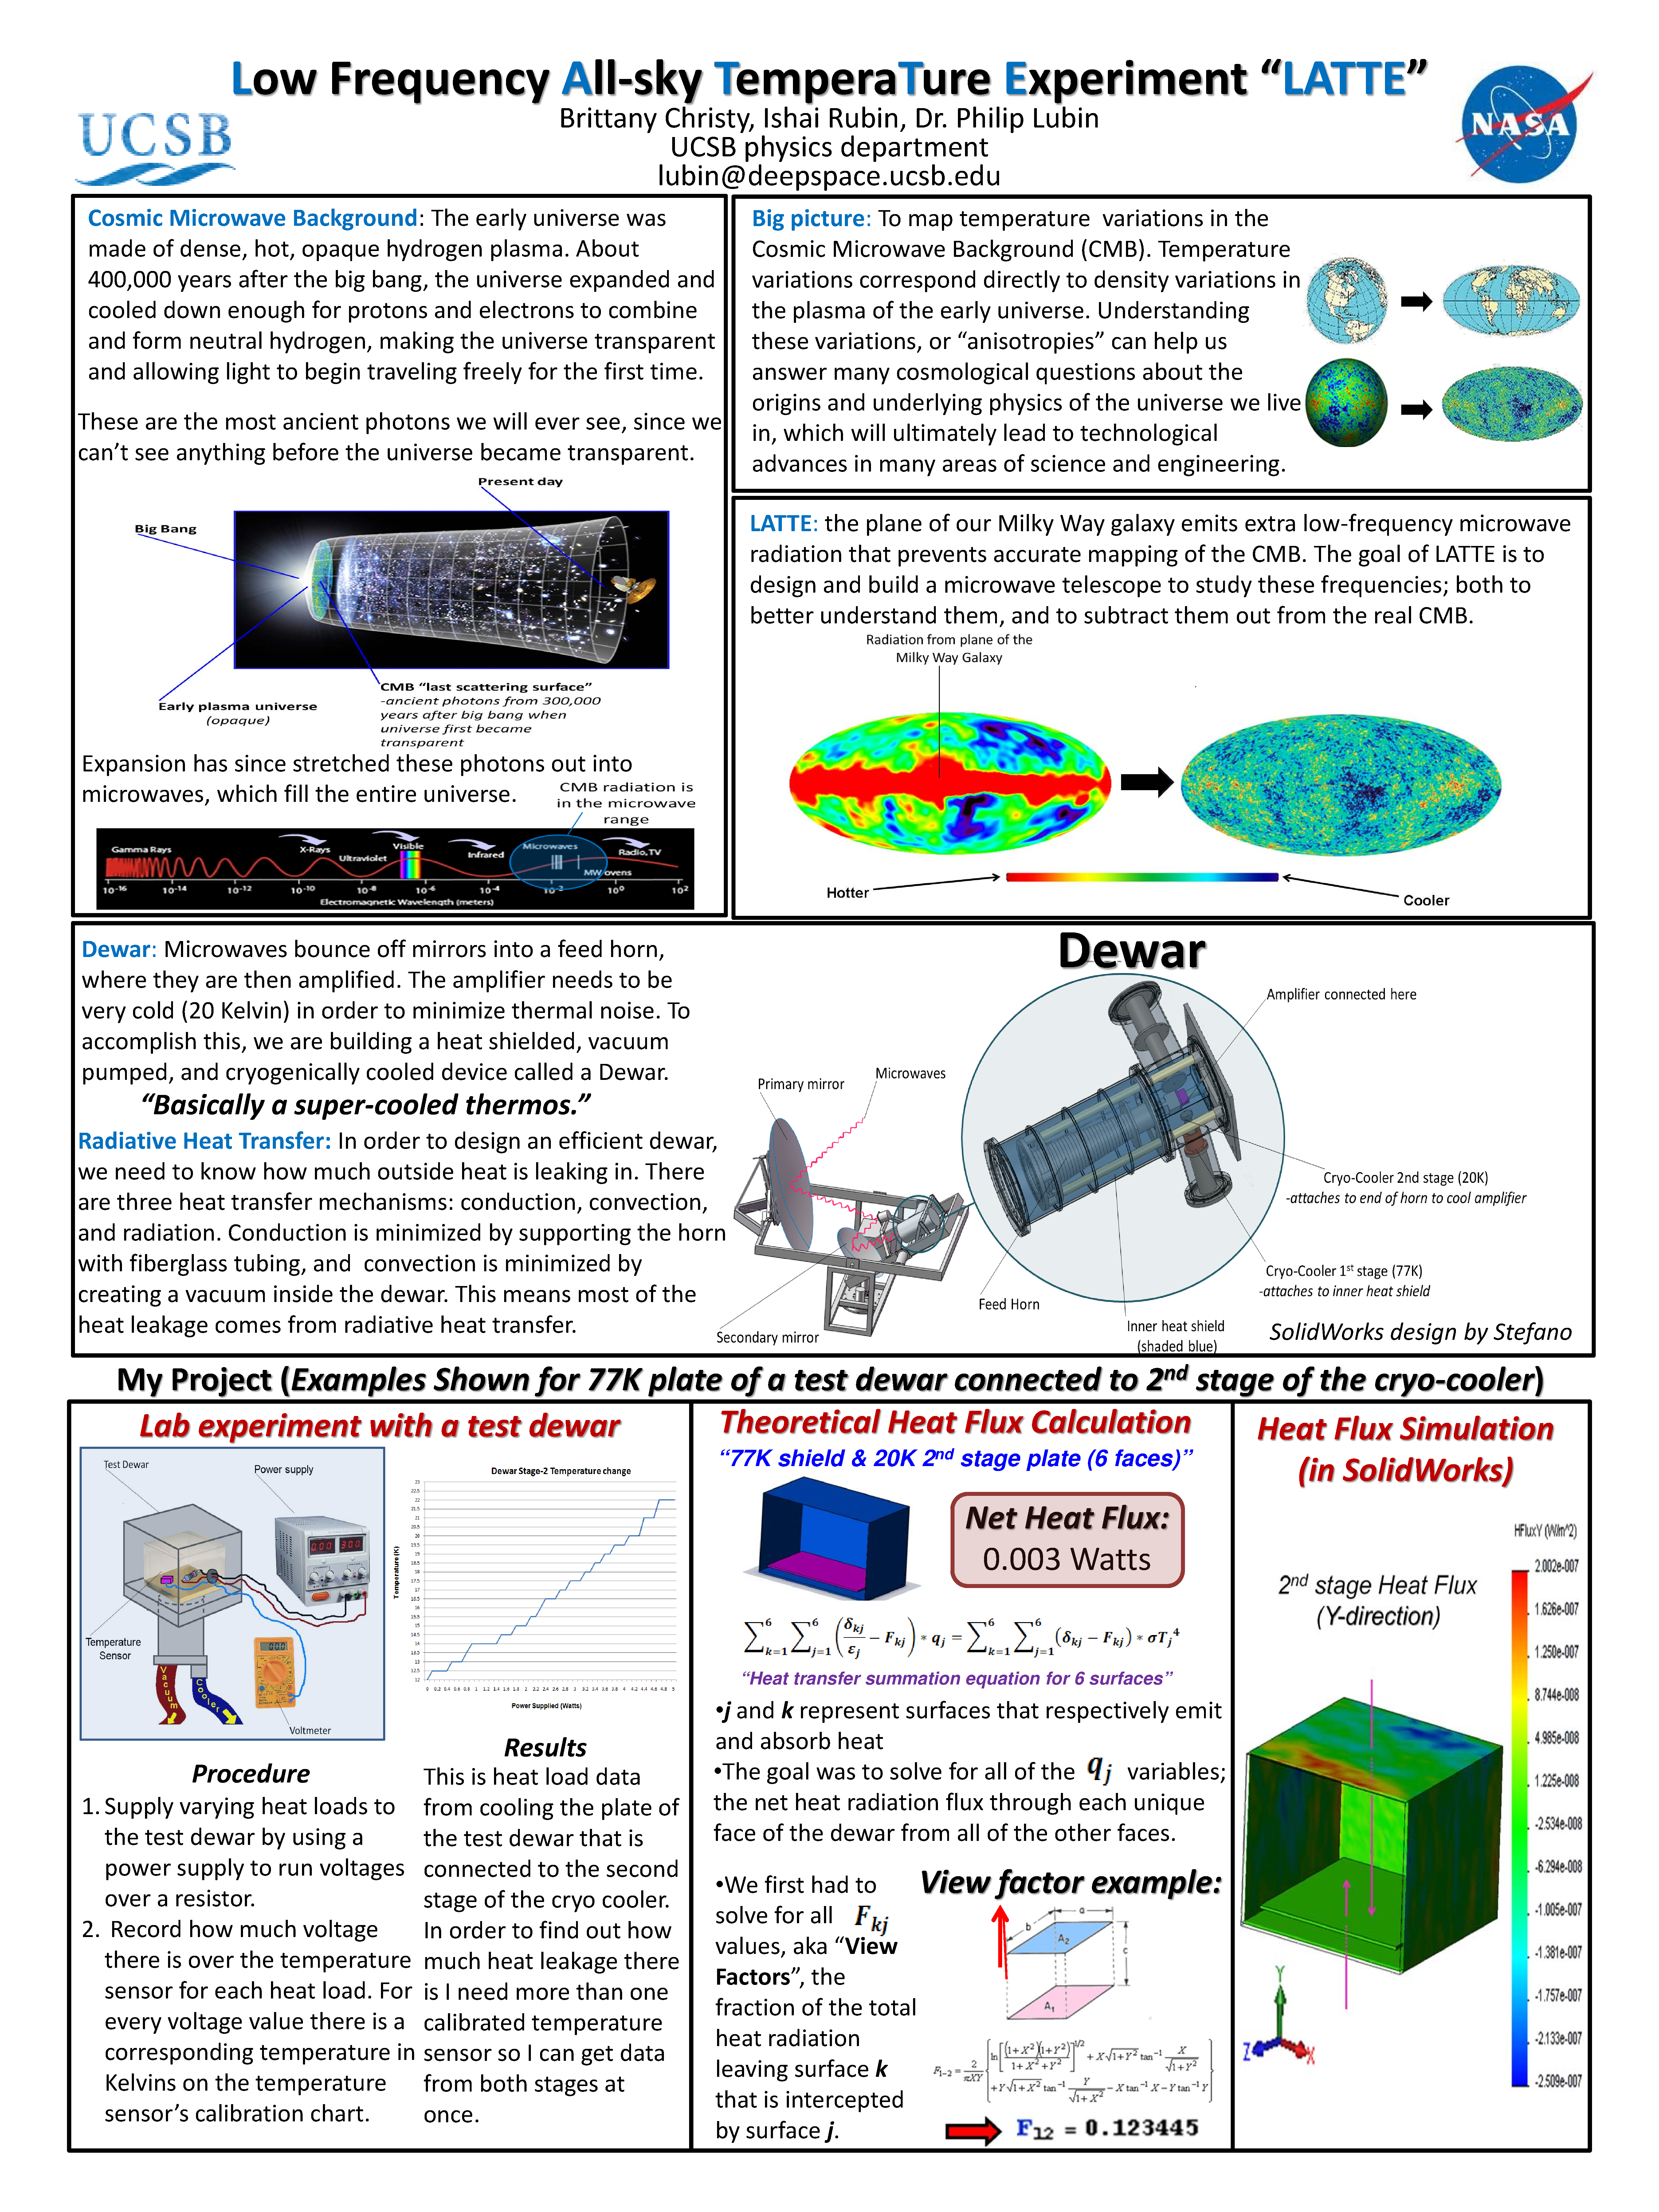
\includepdf[pages=-]{pictures/UCSB/latte_poster.pdf}

\end{document}